\textbf{COLUNI 2024 -- Questão 31}\par\medskip Analise a imagem e o texto a seguir:

\begin{center}\textbf{REGATA DE VOLTA AO MUNDO}\end{center}

\begin{center}
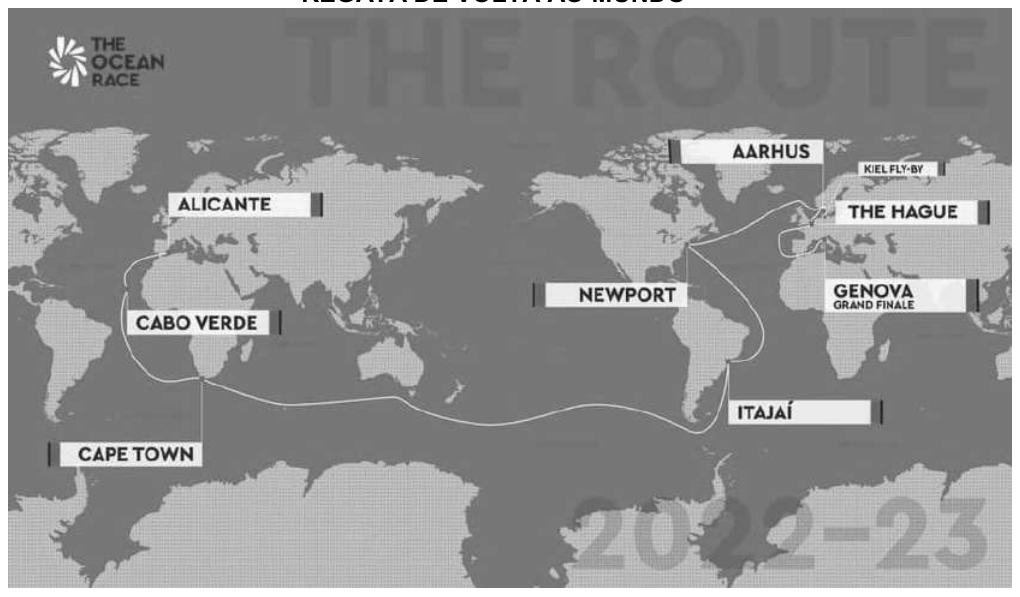
\includegraphics[width=0.78\linewidth,trim=0 0 0 12pt,clip]{static/simulados/coluni/figuras/2024/questao-31/figura-1.png}
\end{center}

Fonte. https://www.lance.com.br/mais-esportes/regata-de-volta-ao-mundo-the-ocean-race-divulga-datas-e-escalas-de-2023.html Acesso em: 01 Ago.2023.

A regata de volta ao mundo é uma prática esportiva que envolve vários espaços geográficos e diferentes paisagens. Considerada a maior regata transoceânica do mundo, a The Ocean Race teve início no dia 15 de janeiro, na cidade espanhola de Alicante e foi finalizada em junho de 2023, na cidade italiana de Gênova.

Sobre esse evento da Geografia do Esporte associado com a cartografia, analise as afirmativas a seguir:

I. A figura apresentada não pode ser tratada como um mapa, por não apresentar de forma clara as coordenadas geográficas e as respectivas escalas.

II. Os fusos horários previstos na regata estão todos no mesmo hemisfério, uma vez que percorrerá apenas o lado ocidental.

III. Trata-se de um evento continental que representa uma nova relação geopolítica, ao aportar em todos os continentes.

IV. A linha internacional da data, marca a passagem dos competidores de um hemisfério para outro, caracterizando a redução de um dia na competição.

Está CORRETO o que se afirma apenas em:
\begin{enumerate}
\item I e IV.
\item II e III.
\item I e III.
\item II e IV.
\end{enumerate}
